\documentclass{article}
\usepackage[b5paper]{geometry}
\usepackage[UTF8]{ctex}
\usepackage{graphicx}

\title{\textbf{Introduction to my search engine system}}
\author{2019201412\quad信息学院\quad向尔格}
\date{\today}

\begin{document}
\maketitle
\section{The functions of the search engine system}
The system crawled 6883 websites from the official website of information institute, renmin university. Users can enter some words or sentences with any length in the input box, and the engine would give top10 relative pages under information institute websites within 1 second.
\section{The design of the system}
I divide the process of creating the system into six steps: 
\begin{enumerate} % for numbers
\item \textbf{Crawl websites (crawl.cpp)} \\
The crawl.cpp is wrote in C++ to run the wget function and violently use system() to call it, then every website's source code is downloaded into ```docid'.txt". \\
For a website, find all the “href” and add new urls which have not been visited to the queue. Using BFS strategy to get all 6883 websites crawled.
\item \textbf{Extract content (extract.cpp)} \\
To remove the redundant contents, through looking for rules, I find it effective to extract all the content between id=``content" and id=``footer". In detail, finding all the pair ``\textgreater" ``\textless", extract the content between `\textgreater'and `\textless', then put all the extracted contents together from former ```docid'.txt' into ```docidext'.txt".
\item \textbf{Cut extracted content (cut.py)} \\
Using jieba in python to cut all the extracted contents into a list of kew words, removing some useless words by part-of-speech analysis. Write the result from ```docidext'.txt" into ```docidcut'.txt"
\item \textbf{Create inverse retrieval (calc\_idf.cpp)} \\
For every word, get every document it appears at and the frequency. Make a pair(docid, frequency) and add it to create the word's retrieval. Write the retrieval information into ``overall.txt"
\item \textbf{Calc scores to find top10 relative doc (Init.cpp)} \\
Using tf-idf strategy to calc documents' scores, then select top10 scored documents.
\item \textbf{Display the result on web UI (app.py)} \\
Using flask to establish communication, cut the query that Users input, run ``Init.cpp" and return top10 relative websites on a beautiful UI.
\end{enumerate}
\section{Some programming skills}
\begin{enumerate}
\item In step 1, I remove some useless websites which has ``.doc", ``.xlsx", ``.pdf", ``ebook" etc.
\item In step 4, I write all the information such as inverse retrieval and document frequency into one file to save time for reading files.
\item In step 6, in home page, I copy baidu.com's source code to display. In the result page, I use some Css(Select.html) to decorate.
\end{enumerate}
\section{Some examples}
First run app.py \\
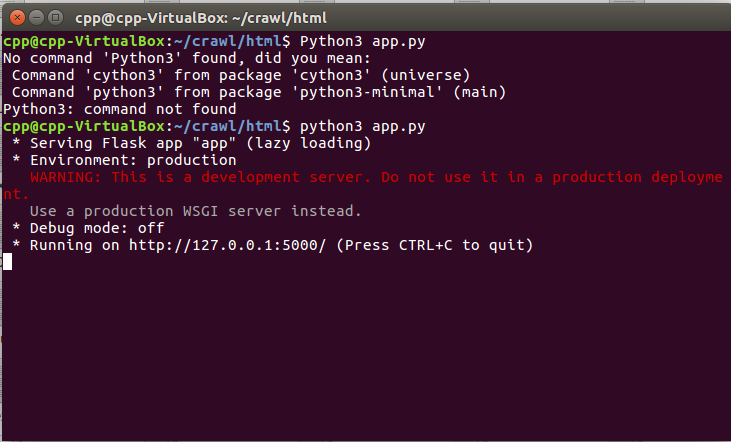
\includegraphics[width=1\textwidth]{start} \\
Users can load into the homepage to input sentences they want to search. \\
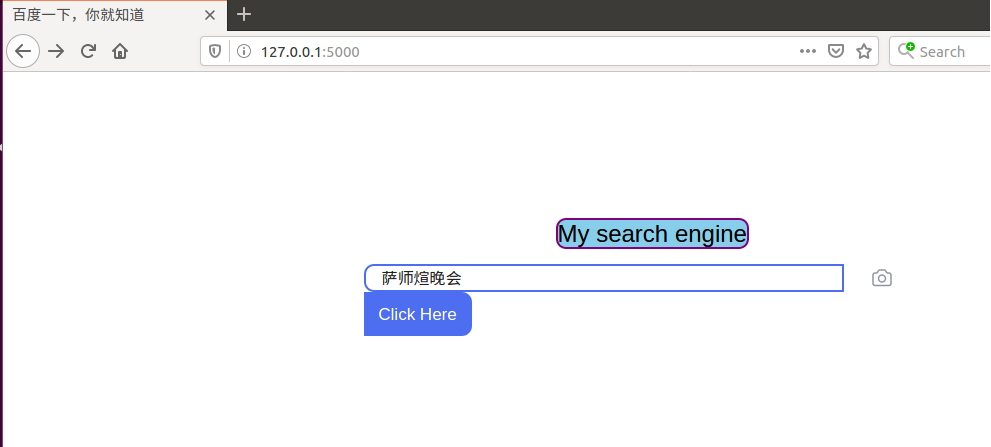
\includegraphics[width=1\textwidth]{home} \\
When Users Click the button, the page will jump to the search result page. \\ 

\includegraphics[width=1\textwidth]{result} \\
The red part is the title of the website, and you can click it to get to the website. The white part is the corresponding abstract contents of the website. The key words would be bold. In my search engine, you can input sentences of any length, the system would quickly deal with them.
\section{Conclusion}
\begin{itemize}
\item Troubles:
\begin{enumerate}
\item The use of fread trouble me for very long time. Not like sprintf, fread would not add `$\backslash$0', so when I use the same array to do the fread, the former information would remain and bring so many problems. The problem directly let my computer get into a dead loop when I crawl, then the Linux system crash. I have to turn to use virtual box.
\item My code style is not very well so some of code is too useless to debug. I'd better to write more functions next time.
\item It would be much quicker to use one language to write all the programs. But I first wrote in C++, then use python, so at last, the system is the combination of the two language. It waste me tons of time and decrease the efficiency of the system.
\end{enumerate}
\item Gains
\begin{enumerate}
\item The program improve my self-learning ability. Many questions which seem to be very difficult exactly are easy to work out through searching and thinking.
\item I learned the importance of planning. “Think twice, code once”, otherwise, would get into embarrassing position
\item It’s significant to distinguish the priorities. Some wrong details could debug later, first figure out the big problem would save much time.
\item Know more knowledge about python and can write simple python program
\item Know more knowledge about html and css
\end{enumerate}
\end{itemize}
It’s a pity that I didn’t have much time to debug to get higher scores. By watching other classmates’ show, I get many useful ways to make my search result more accurate. Now I can refine my system in many different ways. I hope I can perform better in the next program like this.
\section{Usage and arrangement}
All the files are located under one file. When users want to use the search engine, just open the terminal under the file, and run command “python3 app.py”, then turn to page “http://127.0.0.1:5000”, users can input any contents they want to query. The system would quickly return the result to a new page. You can return to the section 4 ``some examples" to see how to use it clearly.
\end{document}
